\documentclass{article}

\usepackage[margin=2cm]{geometry}
\usepackage{graphicx}
\usepackage{fontspec}

\setmainfont{Segoe UI}
\setmonofont{Fira Code}

\title{Matching Engine}
\author{Billy Sumners}

\begin{document}
\maketitle

\section{Introduction}

The Matching Engine is a tool for creating, cancelling, and matching orders for a hypothetical stock at a hypothetical stock exchange. It provides a REST API to achieve these objectives, as well as querying the system for historial orders and trades.

The system will be based around a SQL database. A Spring Boot application will query this database using JDBC, providing a REST API for a web frontend based on React to talk to. Entities will be validated with Spring/Hibernate. Time permitting, there will be an admin frontend based on Thymeleaf.

\section{Database and Entities}

There are four entities considered in this application, represented as tables in the database and classes in the Java application.

\subsection{Database Entities}

\begin{figure}[h]
    \centering
    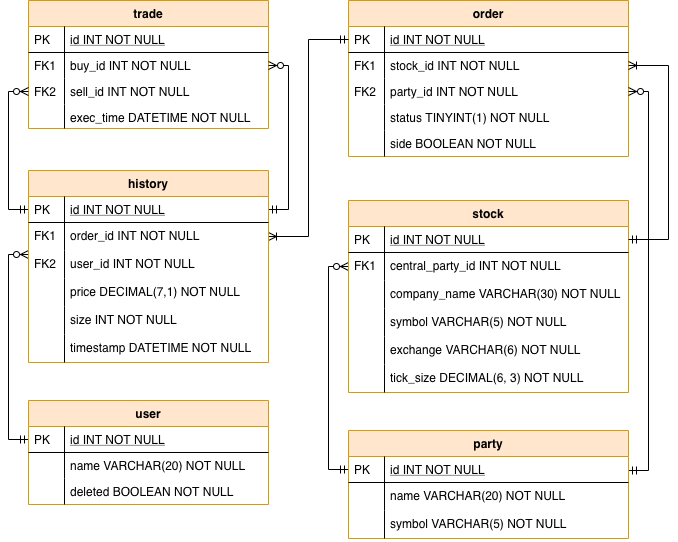
\includegraphics[width=0.7\textwidth]{database-erd.png}
    \caption{Database entity-ralationship diagram}
\end{figure}

\paragraph{Stock} The stock entity corresponds to a stock being traded at the exchange. It has an \texttt{id} to act as the primary key, a \texttt{central\_party\_id} representing the party trading the stock (should be LCH), a \texttt{symbol}, the \texttt{exchange} the stock is traded at, and a \texttt{tick\_size}.

\paragraph{Party} The party entity corresponds to an actual party (e.g. a company) owning the stock. It has an \texttt{id} for the primary key, and a \texttt{name} and \texttt{symbol}.

\paragraph{User} The user entity corresponds to a user working with the application. It has an \texttt{id} to act as the primary key, a \texttt{name} (the username), and a \texttt{deleted} boolean to indicate whether the user is suppressed from the system - deleting the user from the table entirely will break a foreign key constraint with order histories, which we must preserve.

\paragraph{Order} The order entity corresponds to a buy or sell order made in the application. It has an \texttt{id} to act as the primary key, a foreign key \texttt{party\_id} referencing the party owning the stock making the trade, a \texttt{stock\_id} referencing the \texttt{stock} being bought/sold, the \texttt{side} of the order as a boolean (0 = sell, 1 = buy), and the order's \texttt{status}.

Each time an \texttt{order} is made, a new \texttt{history} must be made referencing the initial version of the order.

\paragraph{History} The \texttt{history} entity corresponds to the history of an order's price and size from when it is first created to when the order is fulfilled or cancelled. It has an \texttt{id} to act as the primary key, an \texttt{order\_id} to reference the order, a \texttt{user\_id} to reference the user who made the change to the order (if an order is matched by the system, this will be the user who made the matching order), a \texttt{price}, a \texttt{size}, and a \texttt{timestamp} set to when a \texttt{history} row is made. The idea is that when an order changes its price or size in the  system (through user modification or trades being made), a new version is made.

\paragraph{Trade} The trade entity corresponds to a trade made by the application matching a buy order and a sell order. It has an \texttt{id} to act as the primary key, \texttt{buy\_id} and \texttt{sell\_id} referencing the buy and sell order respectively, and an \texttt{execution\_time} when the trade is made.

\subsection{Java Entities}

\begin{figure}[h]
    \centering
    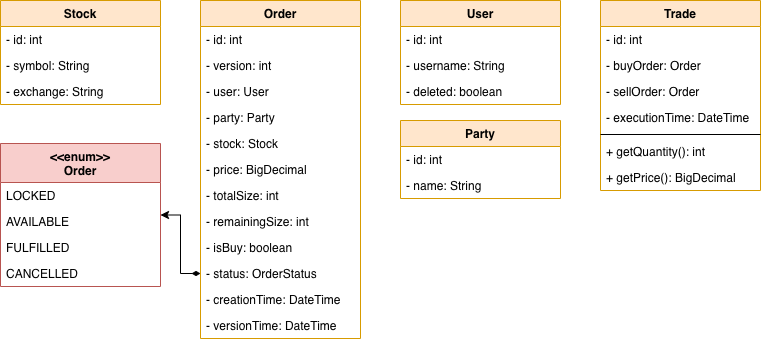
\includegraphics[width=0.7\textwidth]{entities.png}
    \caption{Java entities}
\end{figure}

\paragraph{Stock} The \texttt{Stock} Java class corresponds exactly to the database. A \texttt{Stock} is valid if:
\begin{enumerate}
    \item None of its fields are null.
    \item The \texttt{companyName} has length at most 50.
    \item The \texttt{symbol} has length at most 5.
    \item The \texttt{exchange} has length at most 6.
    \item The \texttt{tickSize} is positive, is at most 100, and has scale at most 3 (i.e. between 0.001 and 100.000).
\end{enumerate}


\paragraph{User} The \texttt{User} Java class corresponds exactly to the database, with \texttt{name} being called \texttt{username} in the class. A \texttt{User} is valid if
\begin{enumerate}
    \item None of its fields are null.
    \item The \texttt{username} has length at most 50.
\end{enumerate}

 
\paragraph{Party} The \texttt{Party} class corresponds exactly to the database. A \texttt{Party} is valid if 
\begin{enumerate}
    \item None of its fields are null.
    \item The \texttt{name} has length at most 50.
    \item The \texttt{symbol} has length at most 5.
\end{enumerate}


\paragraph{Order} The \texttt{Order} class is effectively a combination of the \texttt{order} and \texttt{history} tables. While the \texttt{id} will remain as it is in the database, the \texttt{version} will be calculated based on the position of the version in the \texttt{history} table. The \texttt{versionTime} will correspond to the \texttt{timestamp} in the \texttt{history} table. The \texttt{party\_id} field will be replaced by the referenced \texttt{Party} entity, and the \texttt{stock\_id} will be replaced by the referenced stock entity. The \texttt{price} and \texttt{size} will be as they are in the database. The boolean field \texttt{isBuy} will take the place of \texttt{side} in the table, being \texttt{true} if the order's side is buy, and \texttt{false} if the side is sell. The reason for this design is that it will be easier to commit it to the database, while still remaining somewhat self-documented. An \texttt{Order}'s status will be an enum called \texttt{OrderStatus} which can take five values:

\begin{itemize}
    \item \textbf{\texttt{UNKNOWN} when an order's status is unknown.}
    \item \texttt{EDIT\_LOCK} when an order is being edited.
    \item \texttt{MATCH\_LOCK} when the system finds a matching order and is updating this order in response.
    \item \texttt{ACTIVE} when an order is available for usage.
    \item \texttt{FULFILLED} when the order's size is 0.
    \item \texttt{CANCELLED} when the order has been manually cancelled.
\end{itemize} 
A corresponding state diagram is found in figure \ref{fig:order-state-diagram}.

\begin{figure}[h]
    \centering
    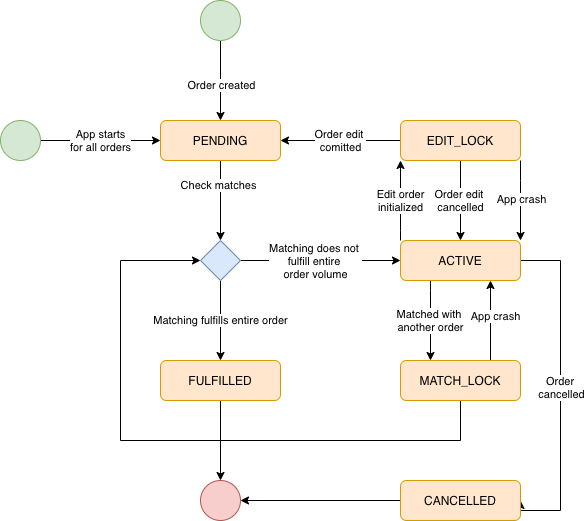
\includegraphics[width=0.7\textwidth]{order-state.png}
    \caption{Order status state diagram}
    \label{fig:order-state-diagram}
\end{figure}

An \texttt{Order} is valid if
\begin{enumerate}
    \item None of its fields are null.
    \item The \texttt{version} is at least 0.
    \item The \texttt{price} is nonnegative, has scale at most 2 and at most 8 digits.
    \item The \texttt{size} is at most 10 000 000.
    \item The \texttt{versionTime} is in the past.
\end{enumerate}


\paragraph{Trade} Within Java, the \texttt{buy\_id} and \texttt{sell\_id} will be replaced by the referenced order entities, with the orders set to be as they were at the time of the trade, \textbf{except for  the \texttt{status}, which will be set to \texttt{UNKNOWN}}. There will be \texttt{getQuantity()} and \texttt{getPrice()} properties, which will be calculated based on the buy order and sell order.

A trade is valid if 
\begin{itemize}
    \item None of its fields are null
    \item The execution time is in the past.
\end{itemize}


\section{Java Backend}

\begin{figure}[h]
    \centering
    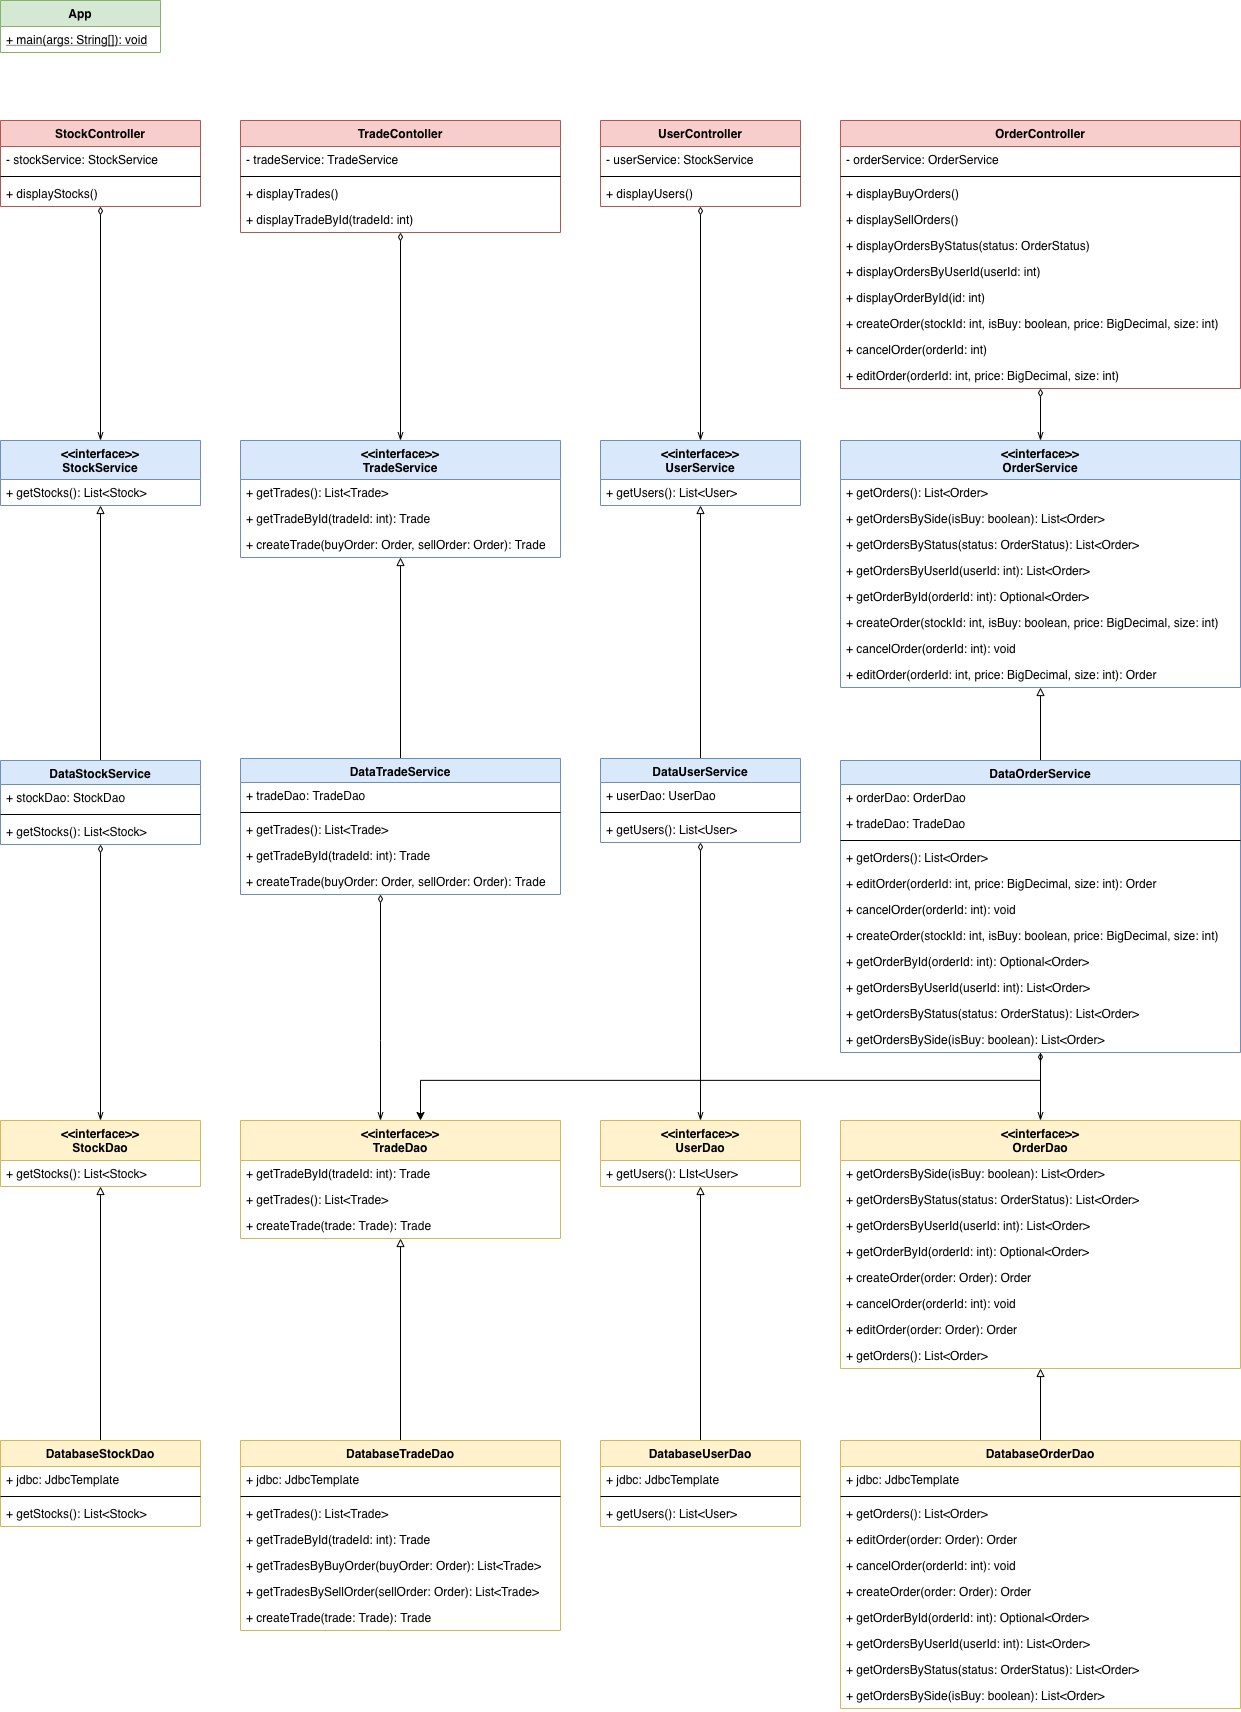
\includegraphics[width=0.9\textwidth]{class-diagram.png}
    \caption{Class diagram}
\end{figure}

The backend is a skyscraper-like design, with classes from controllers down to repositories for each data entity.

\paragraph{Repositories} There are six repositories, one for each data entity, and one for auditing purposes separated into interfaces and implementations. The data entity implementations are prefixed \texttt{Database} to indicate they read to/write from a relational database using \texttt{org.springframework.jdbc.core.JdbcTemplate}. The audit repository implementation is prefixed with \texttt{TextFile} to indicate it writes to a text file.

The \texttt{Stock}, \texttt{User}, and \texttt{Party} DAOs contain a small number of methods as a consequence of being small and mostly immutable entities. In particular, there are methods to get all entities of the relevant type in the system and get an entity by its ID, as well as methods to delete all such entities (primarily for testing purposes), and adding entities. The \texttt{UserDao} also contains a method to edit a user, since a user's \texttt{deleted} field is mutable.

The \texttt{AuditDao} contains only one method, \texttt{writeMessage(message: String)}, whose \texttt{message} parameter contains the message to write to the audit log, to which additional information may be appended by the method.

The \texttt{TradeDao} contains the same add, delete all, get all, and get by ID methods, as well as methods to get a trade by its buy order and its sell order.

The \texttt{OrderDao} contains the same add, delete all, get all, and get by ID methods, as well as including the ability to edit an order, getting all orders by the side they lie on (buy or sell), getting all orders by their status, and getting all orders made by a particular user.

Valdation checks are performed in the DAOs when adding or editing an entity. A specific \texttt{InvalidEntityException} is thrown with a list of validation errors when the checks fail. Editing an entity throws a \texttt{MissingEntityException} when an entity with the ID of the entity in the parameter doesn't already exist in the system.


\paragraph{Services} There are five service classes, one for each entity. The service implementations are prefixed with \texttt{Data} to indicate they talk with a data layer to do their work. Each service implementation communicates with the \texttt{AuditDao} to write down everything that happens in them, as well as the repository corresponding to the entity they manage. The \texttt{DataOrderService} also communicates with the \texttt{TradeDao}.

All services contain passthrough methods delegating to the repository for each method in their entity's repository, except for delete methods. In fact, \texttt{StockService}, \texttt{TradeService}, \texttt{UserService}, and \texttt{PartyService} contain only these methods

The \texttt{OrderService} also contains passthrough methods for its repository, but the \texttt{createOrder(..) and \texttt{editOrder(..)}} methods are slightly special. They take parameters which allow an \texttt{Order} to be constructed, and as it is committed to the repository, the repository checks for any orders of the opposite side matching the committed order, and creates trades/updates orders in response to this. There are also \texttt{beginEditOrder(orderId: int)} and \texttt{cancelEditOrder(orderId: int)}, which update

\section{REST Endpoints}

\subsection{Stock}

\paragraph{GET /stock} Returns a JSON array of all stocks in the system.

\subsection{Trade}

\paragraph{GET /trade} Returns a JSON array of all trades in the system.

\paragraph{GET /trade/\{id\}} Returns a JSON object of a trade in the system with the given ID if it can be found, and 404 not found otherwise. 
 
\subsection{User}

\paragraph{GET /user} Returns a JSON array of all users in the system.

\subsection{Party}

\paragraph{GET /party} Returns a JSON array of all parties in the system.

\subsection{Order}

\paragraph{GET /order/buy} Returns a JSON array of all buy orders in the system.

\paragraph{GET /order/sell} Returns a JSON array of all sell orders in the system.

\paragraph{GET /order/status/\{status\}} Returns a JSON array of all orders with the given status (\texttt{pending}, \texttt{fulfilled}, \texttt{cancelled}). Returns 404 Not Found if the given status does not exist.

\paragraph{\texttt{GET /order/user/\{id\}}} Returns a JSON array of all orders made by the given user, returning 404 Not Found if a user with the given ID does not exist in the system.

\paragraph{\texttt{GET /order/\{id\}}} Returns a JSON object of the order with the given ID, returning 404 Not Found if it cannot be found.

\paragraph{\texttt{POST /order?stock-id=\{stockId\}\&is-buy=\{isBuy\}\&price=\{price\}\&size=\{size\}}} Creates an order in the system with the given parameters, returning a JSON object of the order if it succeeded, and 422 Unprocessable Entity if it did not succeed due to a bad parameter.

\paragraph{\texttt{POST /order/cancel/\{id\}}} Cancels the order with the given ID, returning 404 Not Found if the given order doesn't exist.

\paragraph{\texttt{POST /order/edit/\{id\}?stock-id=\{stockId\}\&is-buy=\{isBuy\}\&price=\{price\}\&size=\{size\}}} Edits an order in the system with the given ID with the given parameters, returning a JSON object of the order if it succeeded, 404 Not Found if the order does not exist, and 422 Unprocessable Entity if it did not succeed due to a bad parameter.

\section{User Frontend}

\end{document} 
